% Created 2026-04-23 Thu 12:08
% Intended LaTeX compiler: lualatex
\DocumentMetadata{lang = en-US,pdfversion = 2.0,pdfstandard = ua-2,tagging = on,tagging-setup = {math/setup=mathml-SE},}
\documentclass[11pt]{article}
\usepackage{amsmath}
\usepackage{fontspec}
\usepackage{graphicx}
\usepackage{longtable}
\usepackage{wrapfig}
\usepackage{rotating}
\usepackage[normalem]{ulem}
\usepackage{capt-of}
\usepackage{hyperref}
\usepackage[margin=1in]{geometry}
\usepackage{fontspec}
\usepackage{verbatim, multicol, tabularx,}
\usepackage{amsmath, amsthm, amssymb, stmaryrd, latexsym, bm, listings, qtree}
\usepackage{framed}
\usepackage{xcolor,colortbl}
\usepackage{media9}
\usepackage[export]{adjustbox}
\usepackage{algorithm}
\usepackage[noend]{algpseudocode}
\usepackage{tikz,pgfplots}
\usetikzlibrary{shapes.geometric}
\let\oldquote=\quote
\let\endoldquote=\endquote
\colorlet{shadecolor}{cyan!15}
\renewenvironment{quote}{\begin{shaded*}\begin{oldquote}}{\end{oldquote}\end{shaded*}}
% From https://tex.stackexchange.com/questions/7032/good-way-to-make-textcircled-numbers
\newcommand*\circled[1]{\tikz[baseline=(char.base)]{\node[shape=circle,draw,inner sep=2pt] (char) {#1};}}
\DeclareMathOperator*{\argmin}{arg\!min}
\DeclareMathOperator*{\argmax}{arg\!max}
\lstset{frame=tb, aboveskip=1mm, belowskip=0mm, showstringspaces=false, columns=flexible, basicstyle={\scriptsize\ttfamily}, numbers=left, frame=single, breaklines=true, breakatwhitespace=true}
\hypersetup{colorlinks=true,urlcolor=blue}
\usepackage{tagpdf}
\tagpdfsetup{activate-all}
\tagpdfsetup{math/alt/use}
\usepackage{polyglossia}
\setdefaultlanguage[variant=en-US]{english}
\author{Christopher Simpkins}
\date{Kennesaw State University}
\title{Artificial Intelligence\\\medskip
\large Heuristic Search}
\hypersetup{
 pdfauthor={Christopher Simpkins},
 pdftitle={Artificial Intelligence},
 pdfkeywords={},
 pdfsubject={Artificial Intelligence Heuristic Search},
 pdfcreator={Emacs 30.2 (Org mode 9.7.11)}, 
 pdflang={English}}
\begin{document}

\maketitle
\section{Informed (Heuristic) Search Strategies}
\label{sec:org041083e}

\begin{itemize}
\item Use domain-specific hints about "distance" from goals
\item Hints encapsulated in a \textbf{heuristic function}, \(h(node)\):

\begin{itemize}
\item \(h(node)\) = estimated cost of cheapest path from \(node\) to a goal state
\item \(h\) is really a function of \(state\), not \(node\).  We use \(h(node)\) to be consistent with \(f(node)\) in best-first search, and path cost, \(g(node)\).
\item Book uses \(f(n)\), \(g(n)\) and \(h(n)\).  I use \(node\) instead of \(n\) to clearly distinguish from \(n\) as an index in problem size, \(N\).
\end{itemize}
\end{itemize}

Example Heuristic for Romania, \(h_{SLD}\):


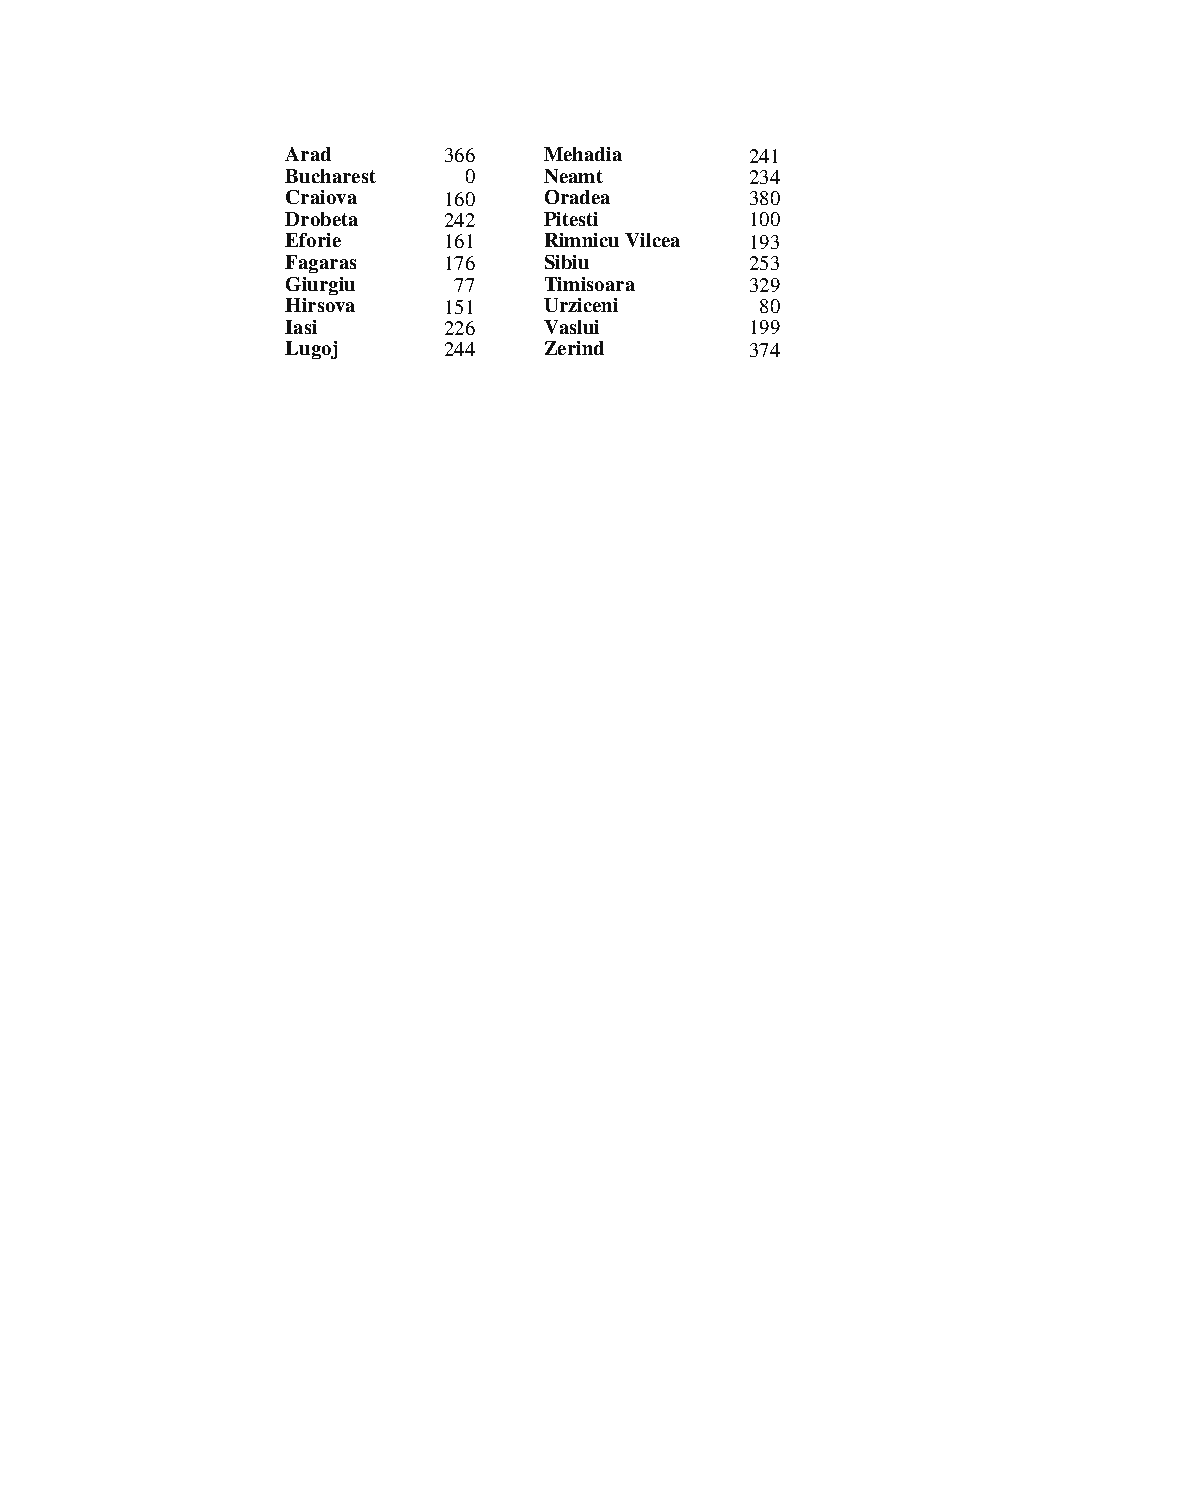
\includegraphics[alt={aima fig 03_16 straight line distances},width=0.75\linewidth]{aima-fig-03_16-straight-line-distances.pdf}


Straight line distances to Bucharest from each of the cities in Romania.
\section{Greedy Best-First Search}
\label{sec:org85e4813}

\begin{itemize}
\item Recall that best-first search uses a priority queue for its frontier, ordered by \(f(node)\)
\item Greedy best-first search uses \(f(node) = h(node)\)
\item Greediness: get as close to the goal as possible in each step
\end{itemize}


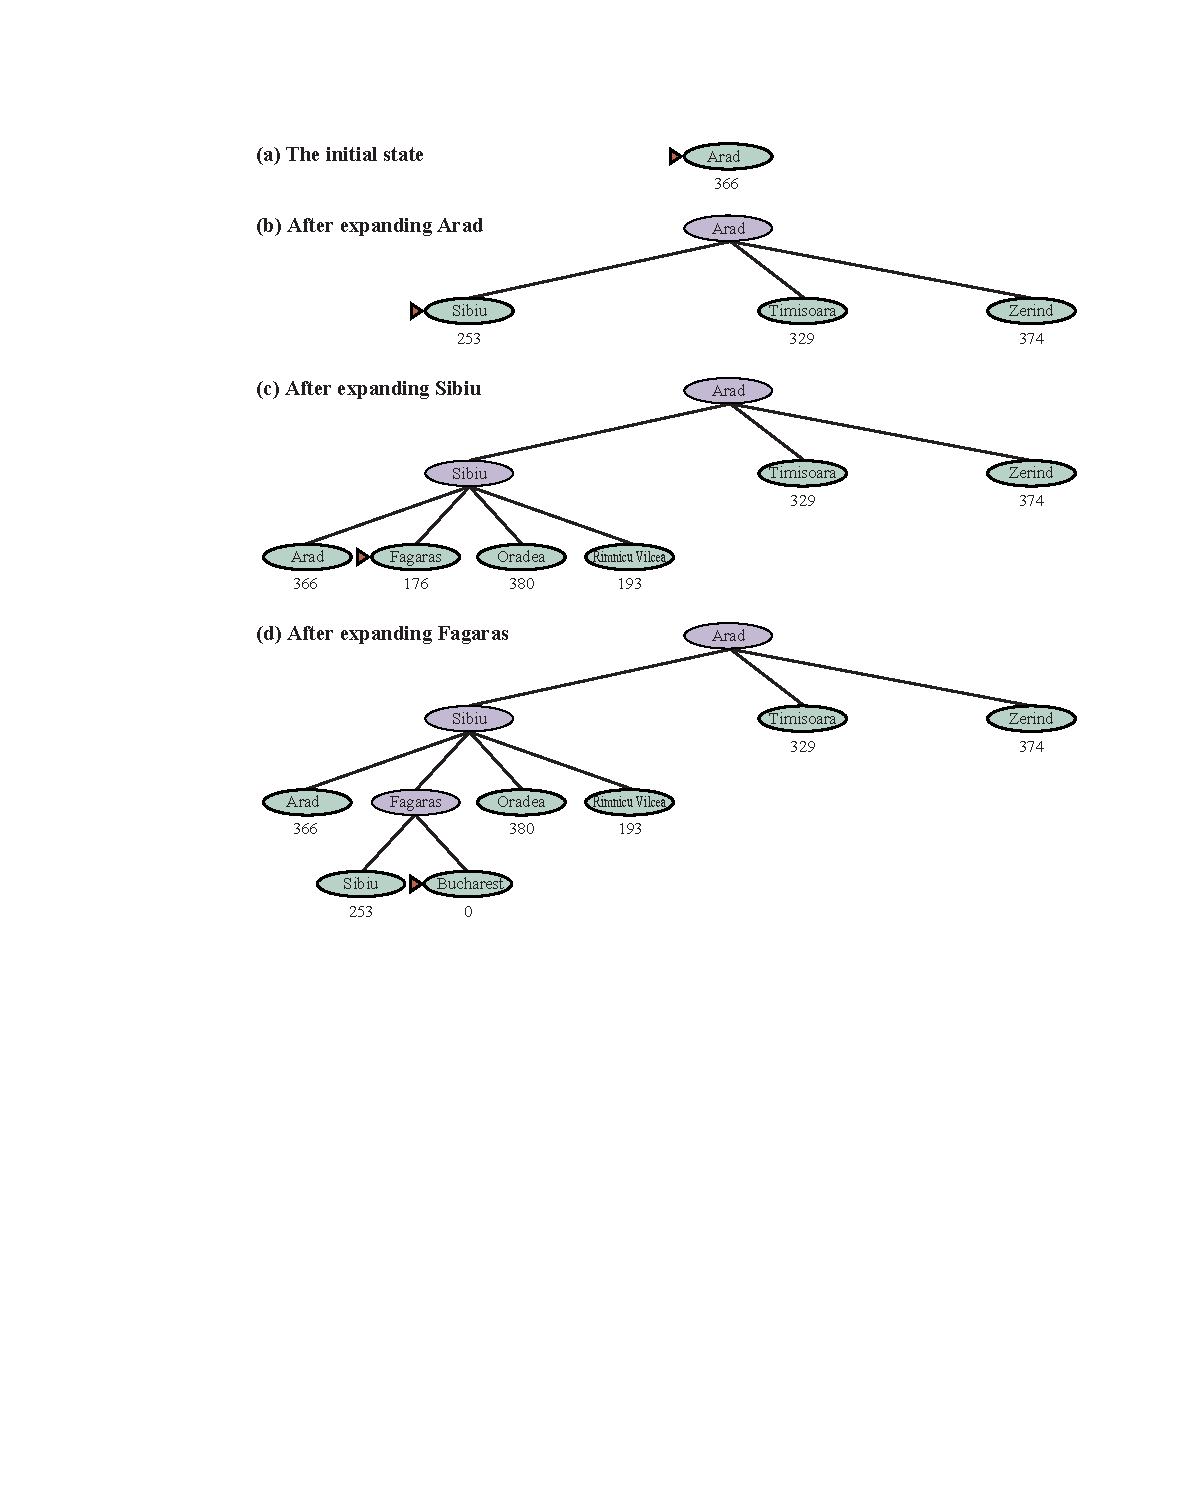
\includegraphics[alt={aima fig 03_17 greedy best first progress},height=2.8in]{aima-fig-03_17-greedy-best-first-progress.pdf}
\section{Optimality of Greedy Best-First Search}
\label{sec:org178581f}


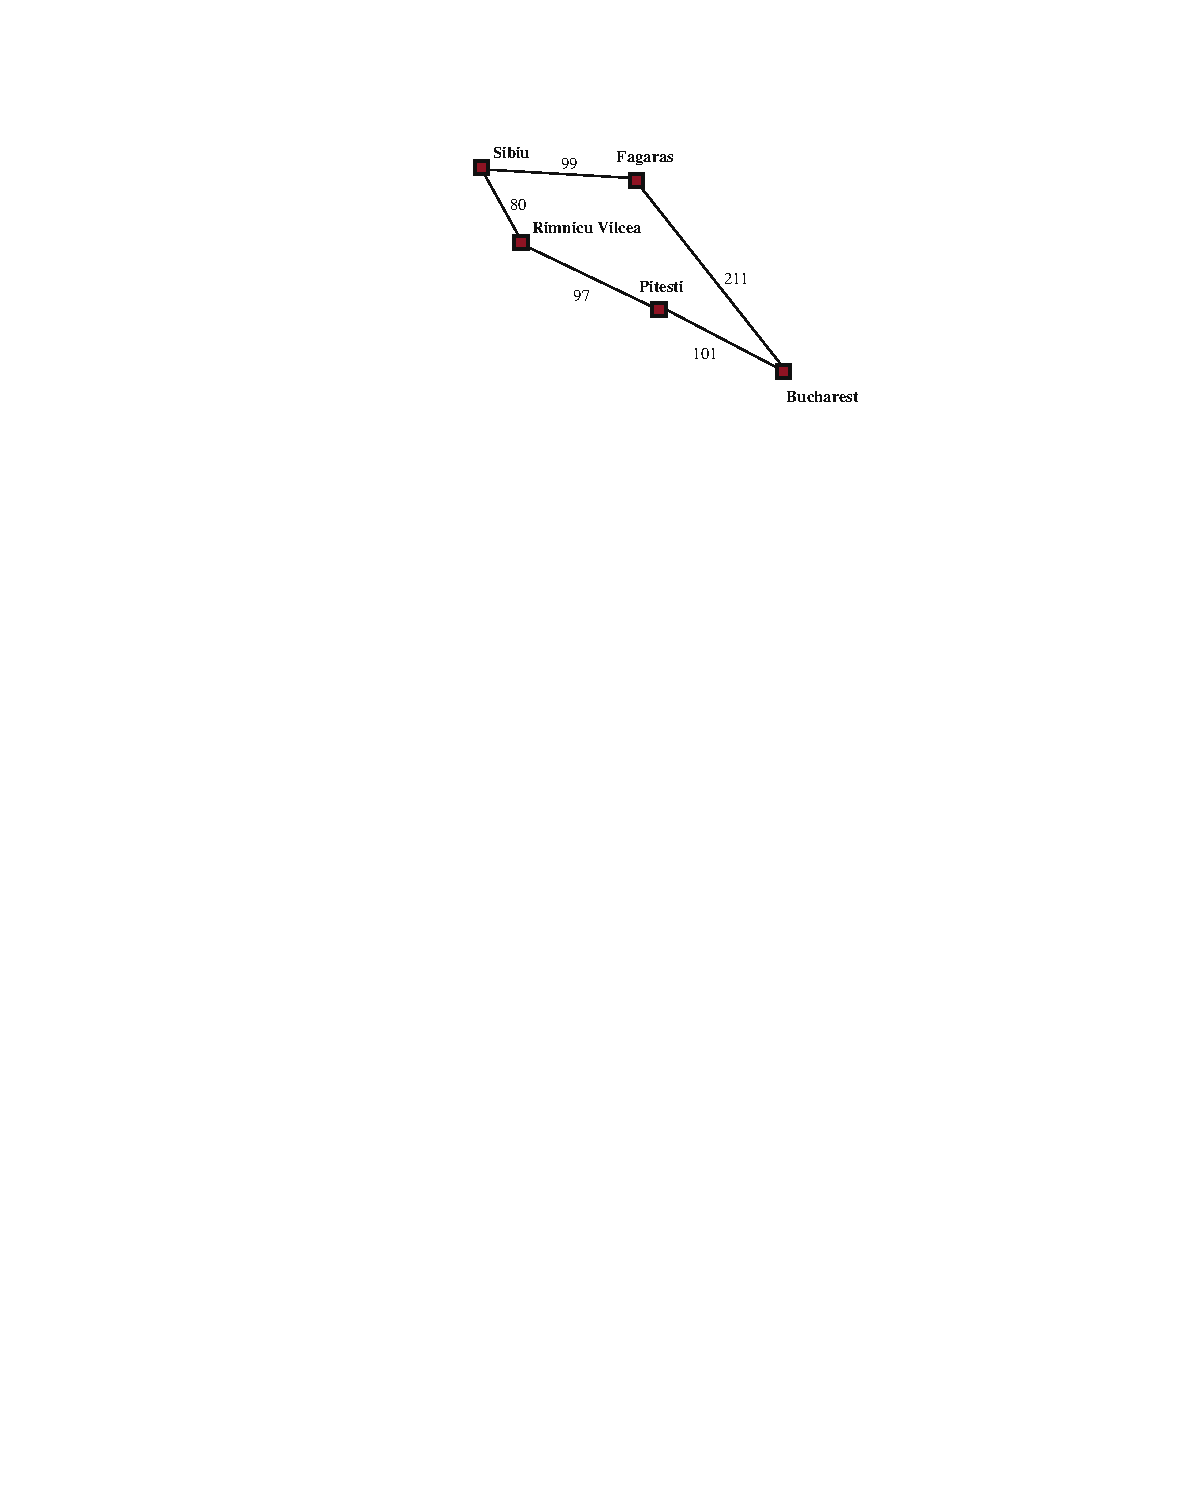
\includegraphics[alt={aima fig 03_10 sibiu bucharest},height=2.0in]{aima-fig-03_10-sibiu-bucharest.pdf}


\begin{itemize}
\item Greedy best-first search returns the path via Sibiu and Fagaras to Bucharest.
\item The path through Rimnicu Vilcea and Pitesti is 32 miles shorter.
\end{itemize}
\section{\(A^*\) Search}
\label{sec:org6c95114}

\begin{equation*}
f(node) = g(node) + h(node)
\end{equation*}

\begin{itemize}
\item Complete
\item Optimal with an admissible heuristic
\item Relatively efficient, but can generate exponential number of nodes for some problems.
\end{itemize}

Heavily dependent on quality of heuristic function.
\section{\(A^*\) Progress Part 1}
\label{sec:org5b34a93}


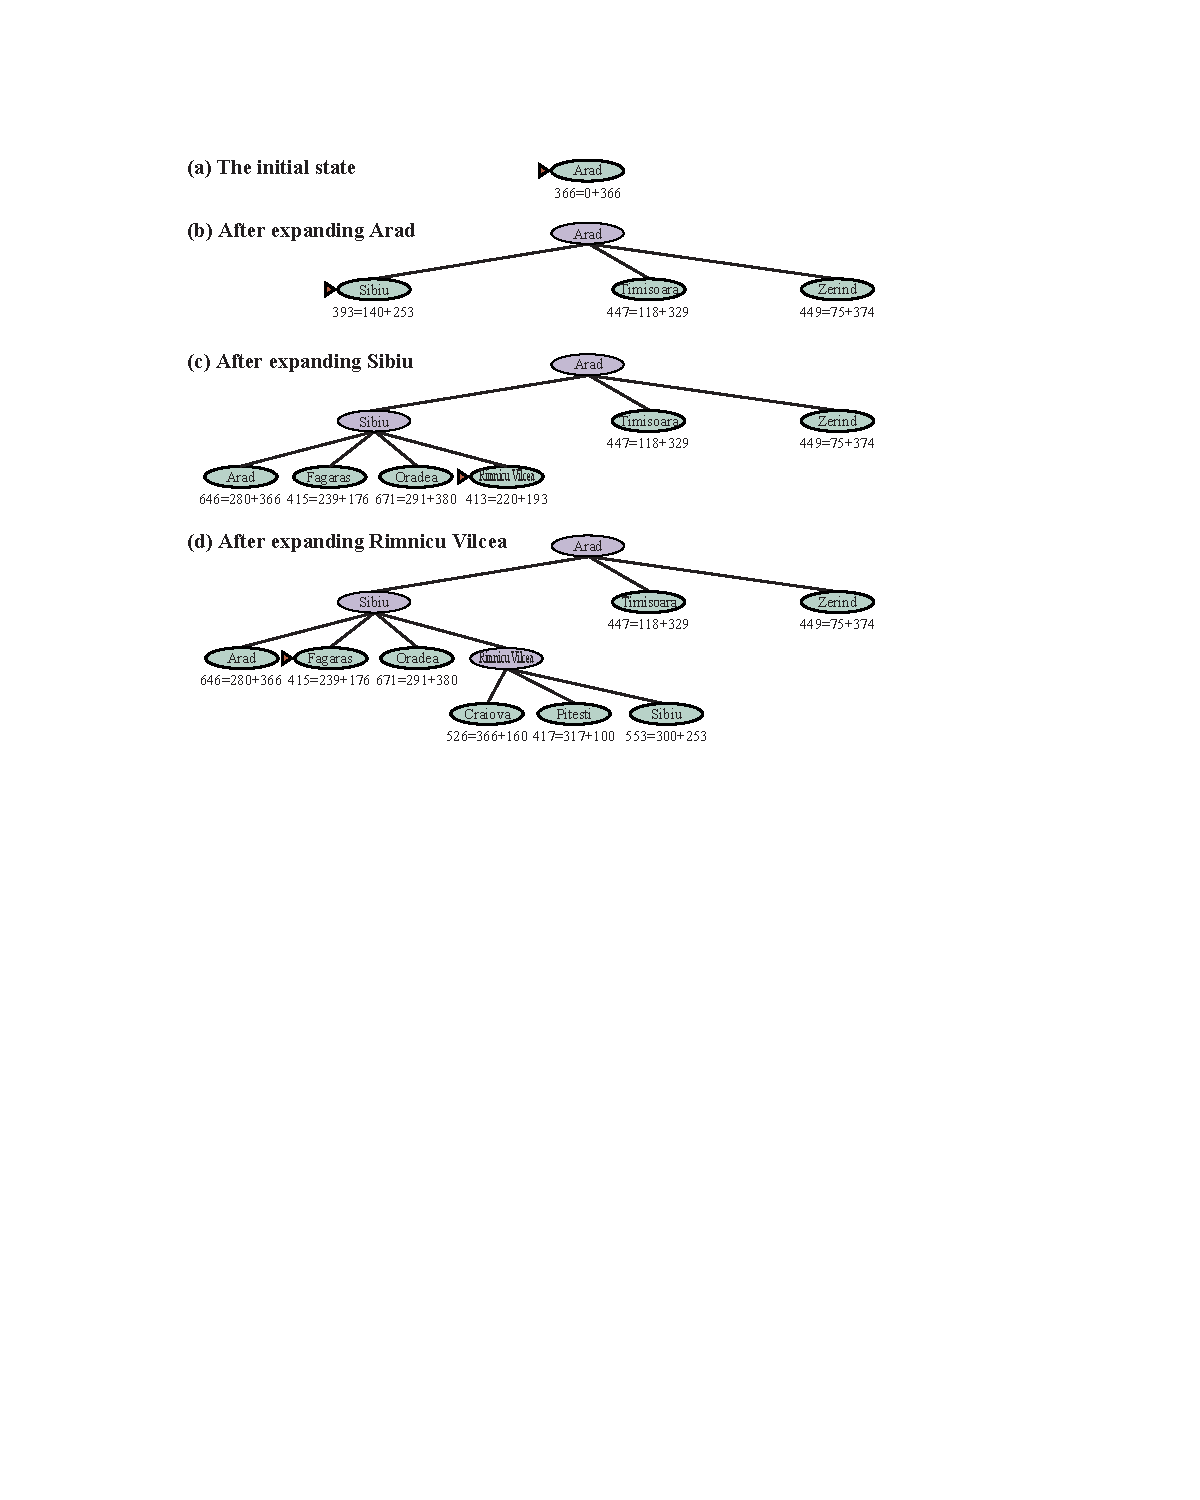
\includegraphics[alt={aima fig 03_18 astar progress 1},height=3.6in]{aima-fig-03_18-astar-progress-1.pdf}
\section{\(A^*\) Progress Part 2}
\label{sec:orgfb7d890}


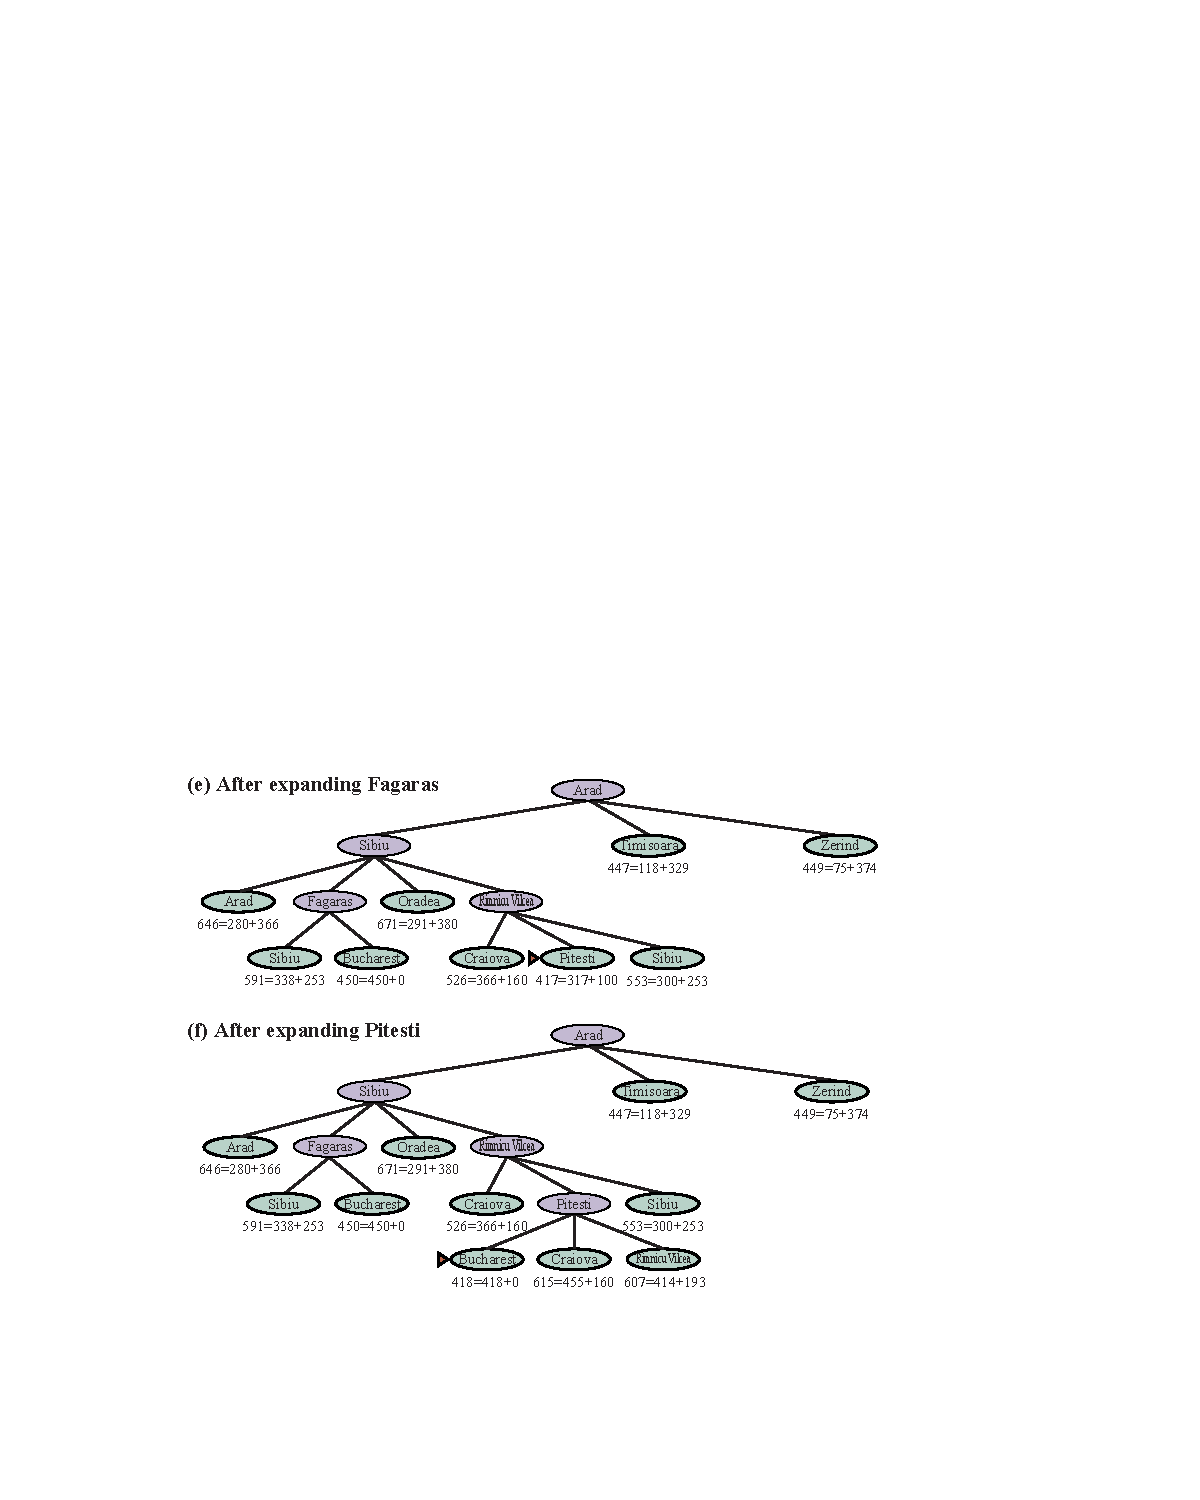
\includegraphics[alt={aima fig 03_18 astar progress 2},width=0.75\linewidth]{aima-fig-03_18-astar-progress-2.pdf}
\section{Admissibility and Consistency}
\label{sec:org2ec75b8}

\begin{itemize}
\item An \textbf{admissible} heuristic never overestimates the cost to reach a goal.
\item A \textbf{consistent} heuristic is a kind of local admissibility: for every node \(node\) and successor \(node'\) generated by action \(a\): \(h(node) \le c(node, a, node') + h(n')\).  This is a form of \textbf{triangle inequality}.
\end{itemize}


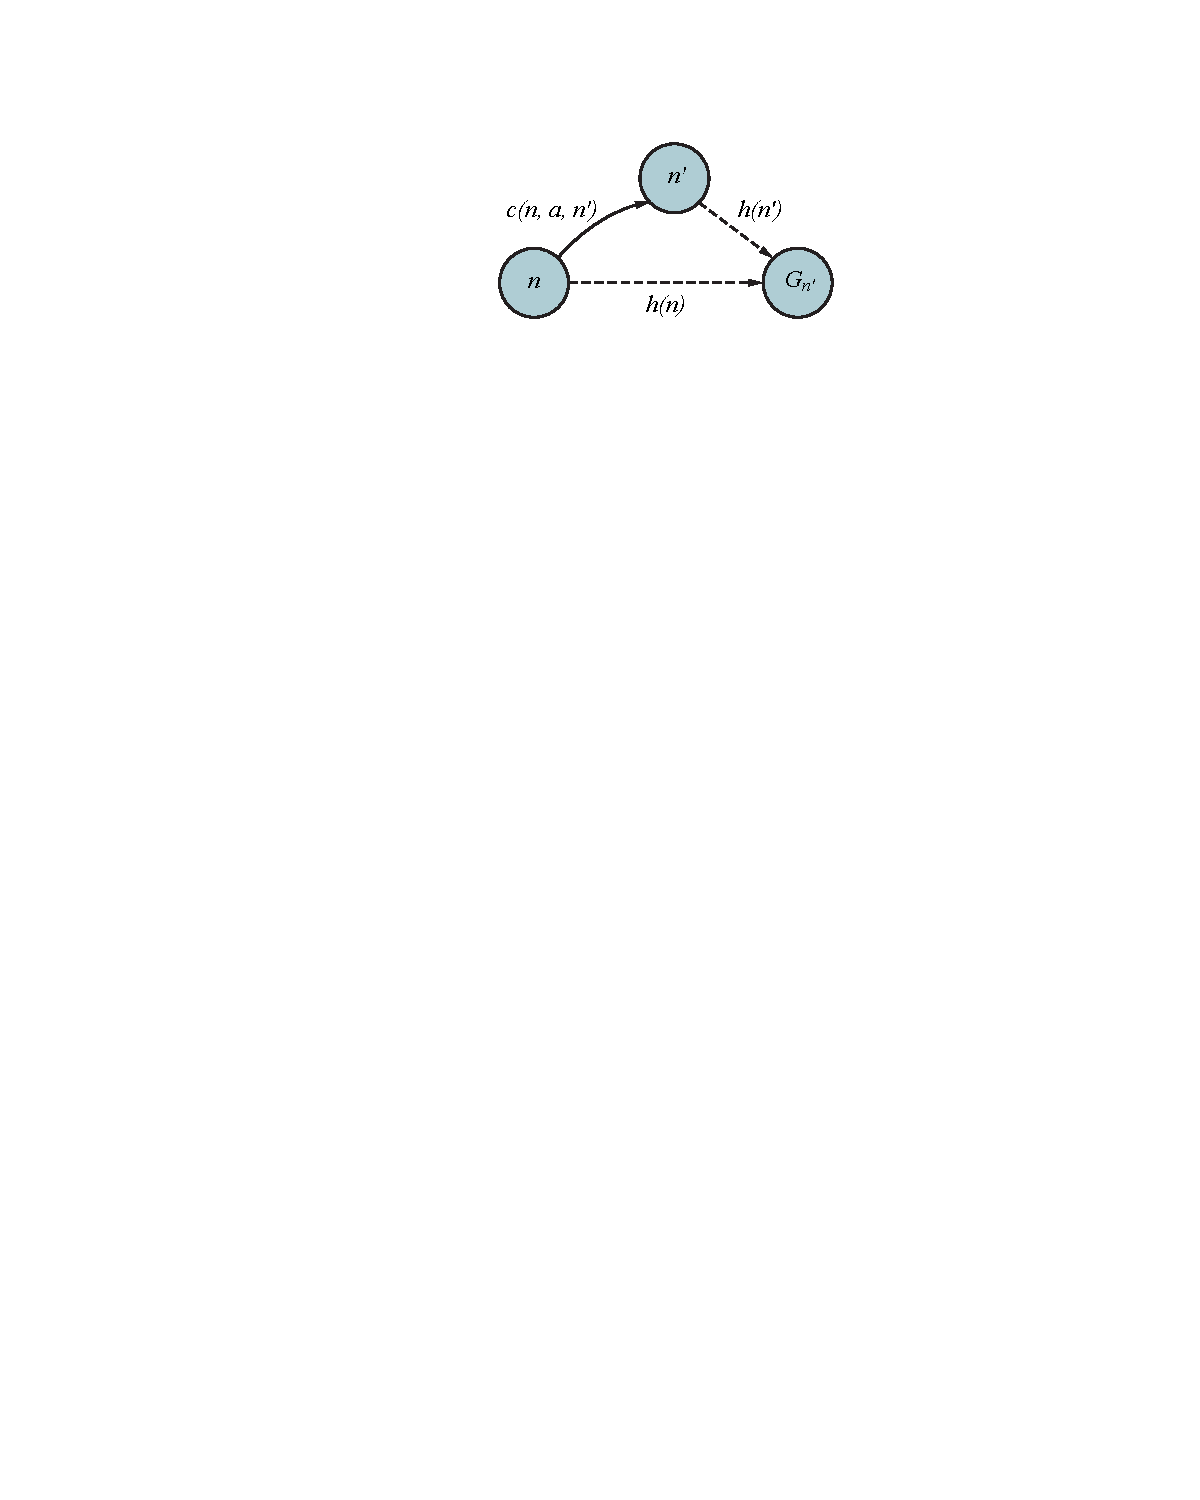
\includegraphics[alt={aima fig 03_19 consistency triangle inequality},width=0.75\linewidth]{aima-fig-03_19-consistency-triangle-inequality.pdf}


\begin{itemize}
\item Admissibility is required to guarantee cost-optimality in \(A^*\).
\item Consistency improves performance by guaranteeing that the first time we reach a node, it is on the optimal path -- so we don't re-evaluate multiple paths to the same node.
\end{itemize}
\section{Satisficing Search: \(A^*\) vs Weighted \(A^*\)}
\label{sec:org6d3acfe}

\begin{itemize}
\item Detour index: multiplier applied to straight-line distance to account for curvature of roads.  E.g., detour index of 1.3 means a road connecting locations 10 miles apart would be estimated as 13 miles long.
\item Weighted \(A^*\) search: apply a wieght, like detour index, to \(h(node)\)

\begin{itemize}
\item \(f(n) = g(n) + w \cdot h(n)\), for some \(w > 1\)
\end{itemize}

\item Results in inadmissible heuristic (overestimates), but can improve search speed.
\end{itemize}



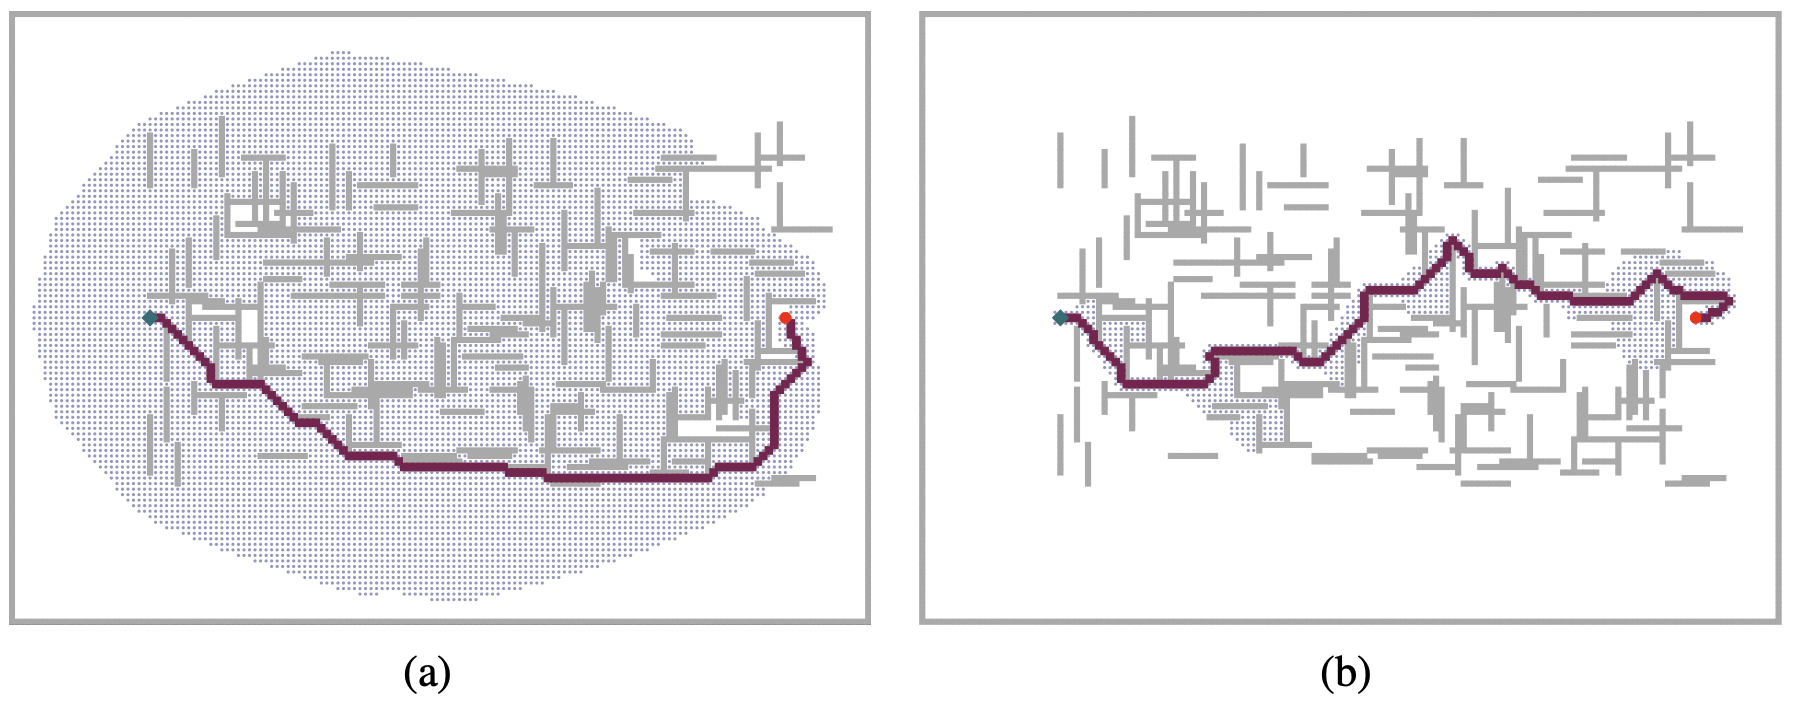
\includegraphics[alt={aima fig 03_21 astar vs weighted astar},height=1.2in]{aima-fig-03_21-astar-vs-weighted-astar.png}


(a) an \(A^*\) search and (b) a weighted \(A^*\) search with weight \(w = 2\).

\begin{itemize}
\item The gray bars are obstacles, the purple line is the path from the green start to red goal, and the small dots are states that were reached by each search.
\item On this particular problem, weighted \(A^*\) explores 7 times fewer states and finds a path that is 5\% more costly.
\end{itemize}
\section{Memory-Bounded Search}
\label{sec:org80aa413}

\(A^*\) is not memory-efficient.  Some approaches to imporoving memory efficiency:

\begin{itemize}
\item \textbf{Beam search}  keeps only the \(k\) nodes with lowest \(f\) values.

\begin{itemize}
\item Forms a narrow "beam" through the search space.
\item Not complete or optimal, but good enough with sufficiently large \(k\)
\item Alternative: keep nodes within \(\sigma\) of best \(f\) score, so only narrow beam when there are clearly better nodes.
\end{itemize}

\item \textbf{Iterative-deepening \(A^*\)} uses \(f = g + h\) as the cut-off for the frontier instead of depth.

\begin{itemize}
\item Iteratively expands contours of search space.
\end{itemize}

\item \textbf{Recursive best-first search} resembles depth-first search.

\begin{itemize}
\item Instead of continuing down a path indefinitely, keeps track of path with second best \(f\) value of ancestor.  If that \(f\) value is exceeded, discards path and backs up to the alternative path.
\item \(f\) value of discarded path is kept in case alternative doesn't work out.
\end{itemize}

\item \textbf{Simplified memory-bounded \(A^*\) (\(SMA^*\))} is similar to RBFS, but expands best leaf node until memory is full.  Then it discards the worst leaf and continues.
\end{itemize}
\section{Search Contours}
\label{sec:org88467b0}

\begin{itemize}
\item In a topographical map, countours indicate a constant elevation
\item In a search contour of a state space, a contour indicates an upper bound on path cost in a region

\begin{itemize}
\item In the 400 countour, each node has \(f(node) = g(node) + h(node) \le 400\).
\end{itemize}
\end{itemize}


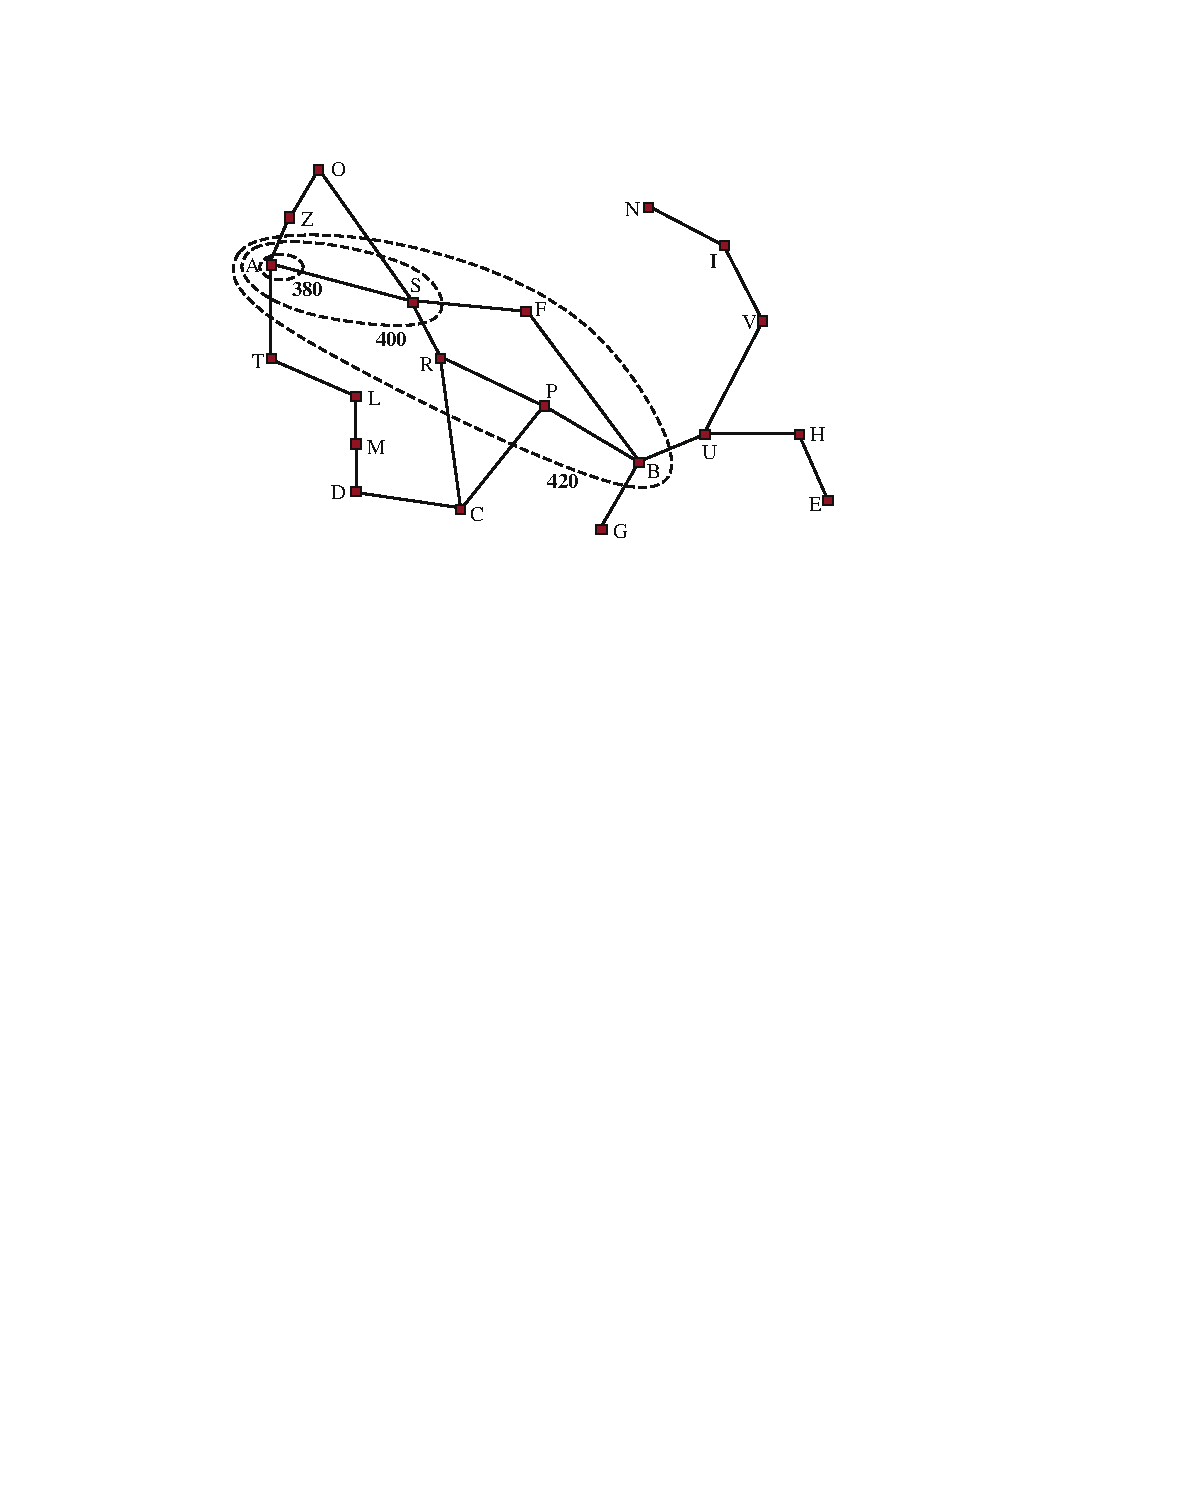
\includegraphics[alt={aima fig 03_20 astar contours},width=0.75\linewidth]{aima-fig-03_20-astar-contours.pdf}


\begin{itemize}
\item Countours represent monotonically increasing path costs.
\end{itemize}
\section{Heuristic Functions}
\label{sec:org38c08ee}


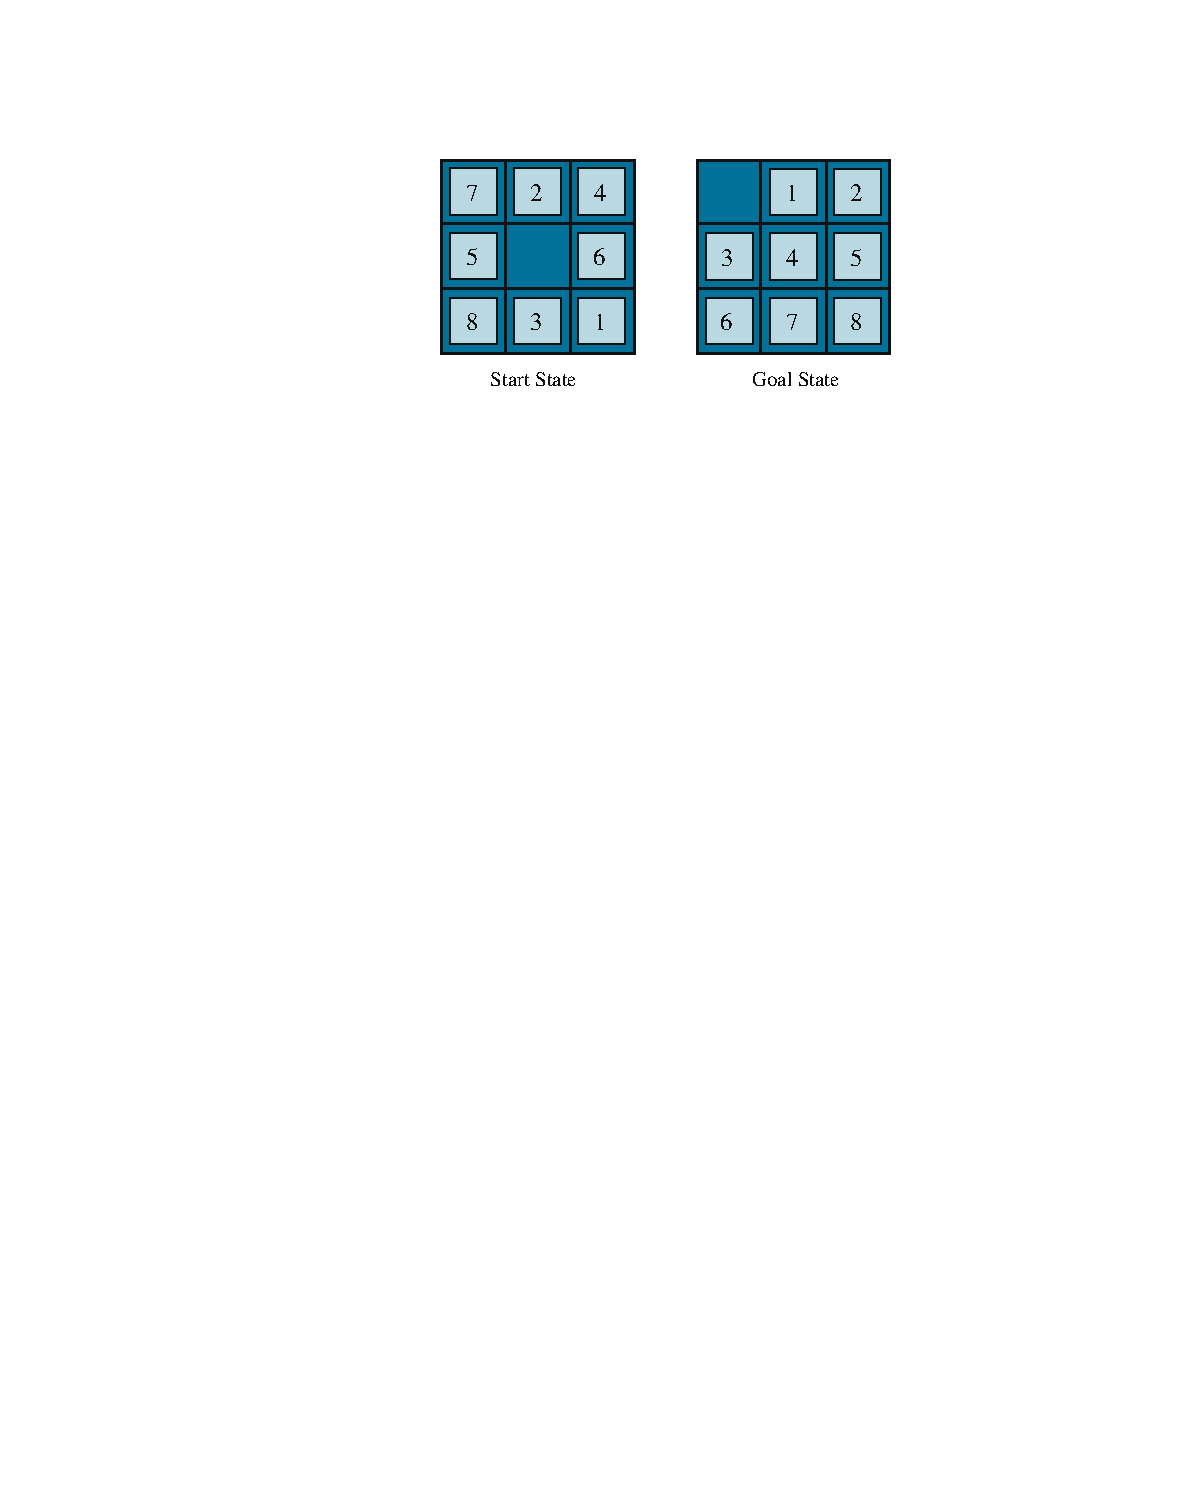
\includegraphics[alt={aima fig 03_03 eight puzzle},width=0.75\linewidth]{aima-fig-03_03-eight-puzzle.pdf}


\begin{itemize}
\item Misplaced tiles, \(h_1 = 8\).
\item Manhattan distance, \(h_2 = 3 + 1 + 2 + 2 + 2 + 3 + 3 + 2= 18\)
\end{itemize}

True solution cost is 26, so neither heristic overestimates.
\section{Heuristic Accuracy and Performance}
\label{sec:org57c5972}

\begin{itemize}
\item Effective branching factor, \(b^*\): for \(N\) nodes, branching factor of uniform tree of depth \(d\) that would contain \(N+1\) nodes.  Want close to 1.

\begin{itemize}
\item \(N + 1 = 1 + b^* + (b^*)^2 + \cdots + (b^*)^d\)
\end{itemize}
\end{itemize}


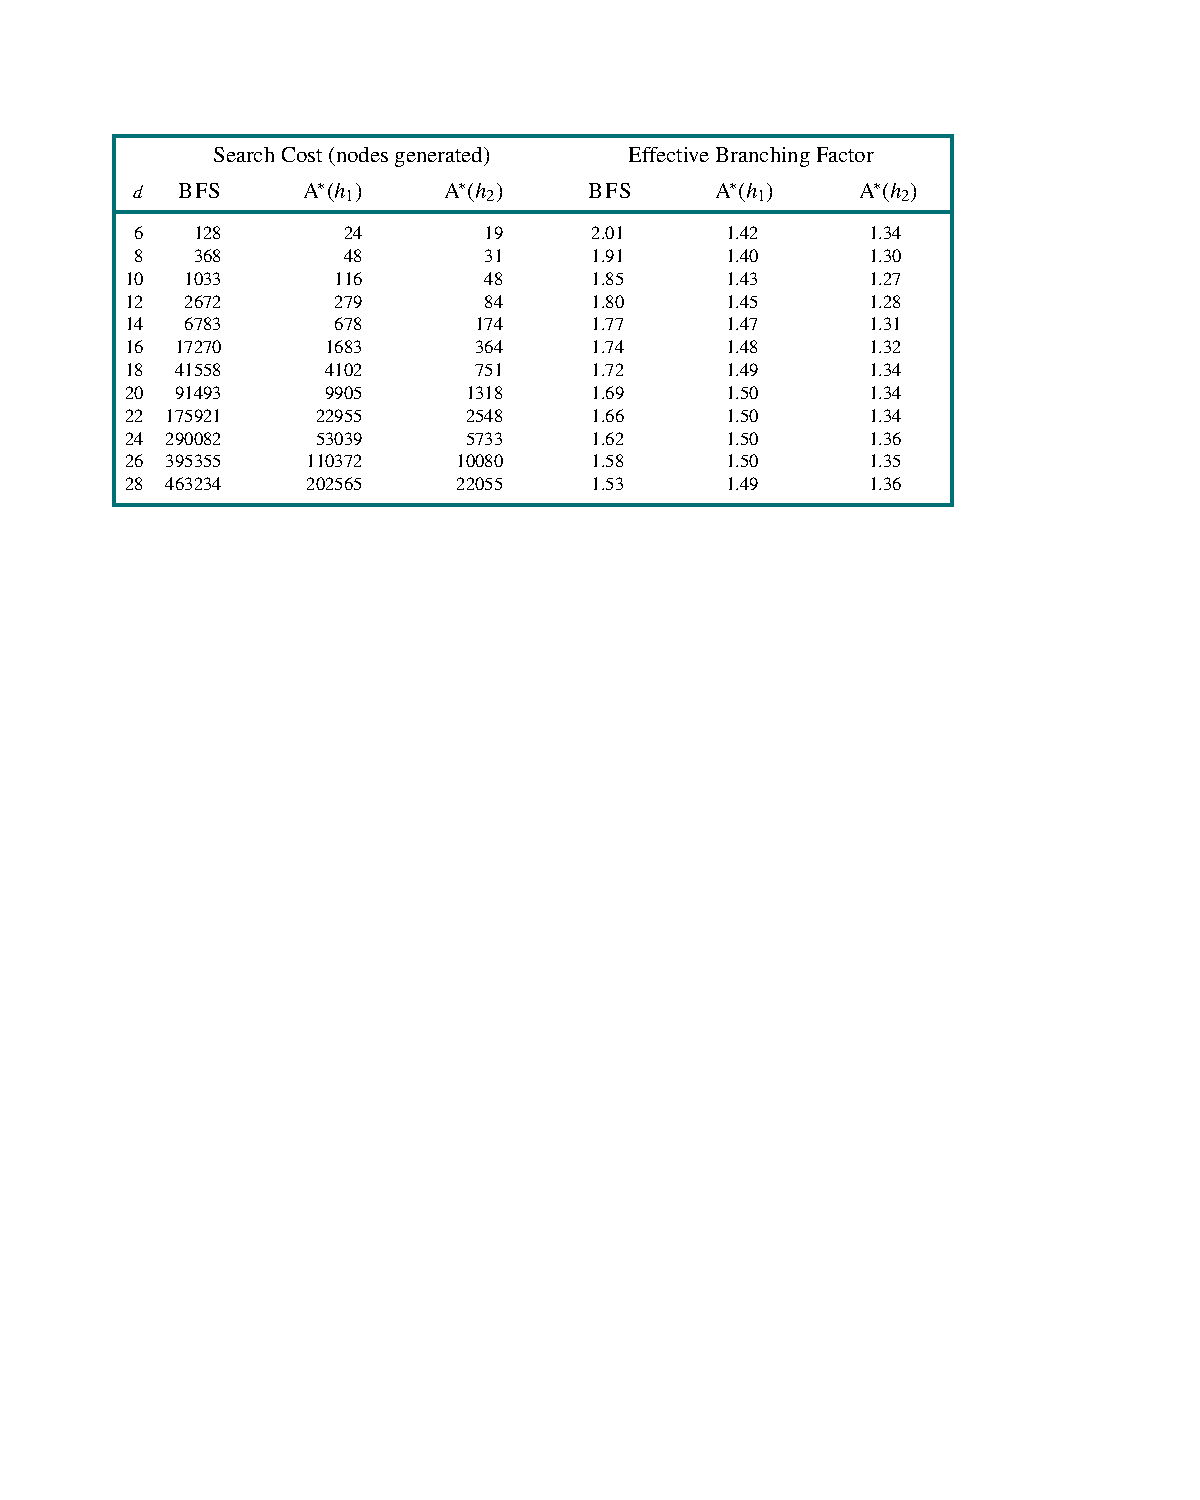
\includegraphics[alt={aima fig 03_26 eight puzzle heuristics comparisons},width=0.75\linewidth]{aima-fig-03_26-eight-puzzle-heuristics-comparisons.pdf}



\begin{itemize}
\item \(h_2\) dominates \(h_1\) because for any \(node\), \(h_2(node) \ge h_1(node)\)
\item We want a heuristic that underestimates, but by as little as possible.
\end{itemize}
\section{Designing Heuristic Functions}
\label{sec:org356aec4}

\begin{itemize}
\item Relaxing the problem definition
\item Storing precomputed solution costs for subproblems in a pattern database
\item Defining landmarks
\item Learning from experience
\end{itemize}

Designing heuristic functions requires domain knowledge.  But there is an automated approach based on relaxed problem definitions: \href{https://www.ijcai.org/Proceedings/91-2/Papers/017.pdf}{\texttt{Absolver}}
\end{document}
